% Look!  A mock introduction

% The introduction is one of the most important pieces of your thesis.  Here is a place for you to introduce the problem(s) on which you have worked and place them in the larger context of your field.  You should aim to ensure that this section is completely understandable to virtually anyone - and certainly anyone with a sophomore-level grasp of physics.  Presumably this will include references to the literature.

% In addition to setting your work into context, a second good idea for your introduction is to give a short outline for what the rest of your thesis will discuss.  This is often done in the closing paragraph(s) of the introduction with sentences like ``In the following chapters \ldots " and ``Chapter 2 discusses \ldots"  Tremendous detail is not required in this outline, but rather just a brief road map for the rest of the document.

This thesis centers on the modeling of Passive Daytime Radiative Cooling Devices (PDRCs) utilizing the COMSOL Multiphysics™ software. PDRCs exhibit a unique capability to dissipate blackbody radiation, transferring energy to the cold reservoir of outer space without requiring electrical input. Consequently, PDRCs hold the promise of addressing two significant challenges: the energy crisis and global warming. % rephrased

\section{Cooling is Critical}
Over the years, cooling has become more critical to humans due to global warming, rapid population growth and industrial development. Various methods exist for cooling buildings, ranging from traditional practices such as shading and solar orientation to the use of electric fans. The most advanced approach is air conditioning (AC), encompassing systems that enhance indoor thermal comfort and air quality. While mechanical cooling techniques date back to the 19th century, widespread adoption of air conditioning began in the 1950s, driven by improved performance, affordability, and economic prosperity, primarily in the United States. Modern air conditioning systems vary widely in size and cost, catering to individual rooms or entire buildings, with electricity being the predominant power source. Urban areas, both in industrialized nations and emerging economies, predominantly house the majority of cooling systems in use today. 
% (CHEN ET AL. 2021) AND (INTERNATIONAL ENERGY AGENCY, 2018).

Global sales of air conditioners (ACs) have exhibited consistent growth in recent years. Over the period from 1990 to 2016, annual AC sales experienced a nearly fourfold increase, reaching 135 million units. In 2016, China emerged as the leading market in terms of AC capacity sales, totaling nearly 390 gigawatts (53 million units). % rephrased

\begin{figure}
  \centering
  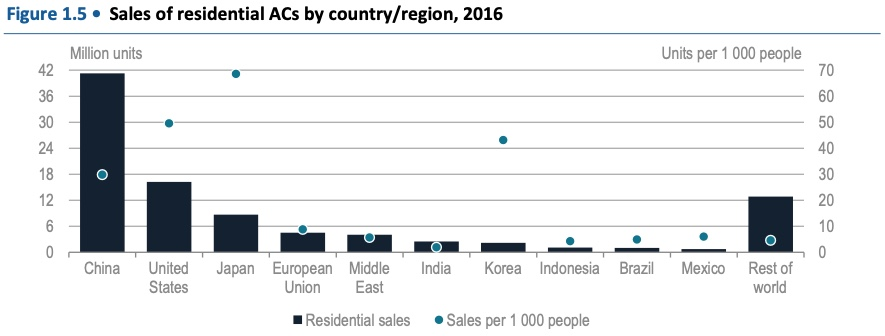
\includegraphics[width=0.8\textwidth]{Chapters/Figures/Sales of Residential ACs by Country or Region, 2016.jpg}
  \caption{Sales of Residential ACs by Country or Region, 2016}
\end{figure}

The growing demand for cooling is significantly influencing power systems, primarily due to the reliance on electricity-driven fans or air conditioners to meet cooling requirements. The escalating demand for air conditioning, in particular, not only elevates overall electricity consumption but also contributes to higher peak electricity loads. Additionally, the emission of greenhouse gases (GHGs) from ACs occurs through refrigerant leakage or improper disposal. It's noteworthy that these refrigerants are potent GHGs with adverse implications for climate change. % (INTERNATIONAL ENERGY AGENCY, 2018) % rephrased

Improving the efficiency of air conditioning systems (ACs) is pivotal in mitigating peak electricity demand, thereby resulting in decreased emissions and associated financial implications. Endeavors focused on enhancing cooling efficiency necessitate a thorough assessment of the comparative costs linked to diverse cooling technologies. % rephrased

\section{Radiative Cooling}
Objects with temperatures above absolute zero emit blackbody radiation across all wavelengths. Radiative passive cooling occurs when objects emit more blackbody radiation than they absorb, resulting in a temperature reduction below the ambient level. The surplus emitted heat is transferred to outer space through thermal radiation, leveraging the substantial temperature contrast between Earth (approximately 300 K) and outer space (approximately 3 K). This process efficiently exchanges heat with the infinite cold reservoir of deep space, achieving cooling without any energy consumption. % rephrased

Passive radiative cooling can be realized during the daytime, necessitating precise tuning of optical properties across a broad spectrum of wavelengths, from ultraviolet to mid-infrared. As a result, achieving effective passive radiative cooling imposes stringent requirements on materials and structures to mitigate solar heating: % rephrased

\begin{figure}
  \centering
  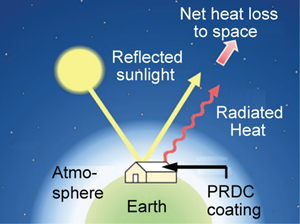
\includegraphics[width=0.4\textwidth]{Chapters/Figures/Schematic for Radiative Cooling.png}
  \caption{Schematic for Radiative Cooling}
\end{figure}

\begin{enumerate}
\item 0\% absorptivity/$\alpha$ (100\% reflectance/$R$) in the solar spectrum (0.3–2.5 $\mu m$), so the surface is not heated by sunlight in daytime at all.
\item Emittance ($\varepsilon$) of 1 in the so-called long-wavelength infrared (LWIR) transmission window of the atmosphere ($\lambda$ = 8–13 $\mu m$), where the atmosphere is partially transparent, since there is limited infrared absorption by gas molecules.
\item $\varepsilon$ of 0 in other mid-infrared wavelengths (e.g., 5–8 $\mu m$ and $>$13 $\mu m$). This is because the atmosphere is not transparent in these ranges.
\end{enumerate}
